\documentclass{beamer}
\usepackage[utf8]{inputenc}

\usetheme{Madrid}
\usecolortheme{default}
\usepackage{amsmath,amssymb,amsfonts,amsthm}
\usepackage{txfonts}
\usepackage{tkz-euclide}
\usepackage{listings}
\usepackage{adjustbox}
\usepackage{array}
\usepackage{tabularx}
\usepackage{gvv}
\usepackage{lmodern}
\usepackage{circuitikz}
\usepackage{tikz}
\usepackage{graphicx}

\setbeamertemplate{page number in head/foot}[totalframenumber]

\usepackage{tcolorbox}
\tcbuselibrary{minted,breakable,xparse,skins}



\definecolor{bg}{gray}{0.95}
\DeclareTCBListing{mintedbox}{O{}m!O{}}{%
  breakable=true,
  listing engine=minted,
  listing only,
  minted language=#2,
  minted style=default,
  minted options={%
    linenos,
    gobble=0,
    breaklines=true,
    breakafter=,,
    fontsize=\small,
    numbersep=8pt,
    #1},
  boxsep=0pt,
  left skip=0pt,
  right skip=0pt,
  left=25pt,
  right=0pt,
  top=3pt,
  bottom=3pt,
  arc=5pt,
  leftrule=0pt,
  rightrule=0pt,
  bottomrule=2pt,
  toprule=2pt,
  colback=bg,
  colframe=orange!70,
  enhanced,
  overlay={%
    \begin{tcbclipinterior}
    \fill[orange!20!white] (frame.south west) rectangle ([xshift=20pt]frame.north west);
    \end{tcbclipinterior}},
  #3,
}
\lstset{
    language=C,
    basicstyle=\ttfamily\small,
    keywordstyle=\color{blue},
    stringstyle=\color{orange},
    commentstyle=\color{green!60!black},
    numbers=left,
    numberstyle=\tiny\color{gray},
    breaklines=true,
    showstringspaces=false,
}
%------------------------------------------------------------

\title
{4.8.30}
\author 
{AI25BTECH11034 - Sujal Chauhan }



\begin{document}

\frame{\titlepage}
\begin{frame}{Question}

Find the equation of a line passing through the point (2,3,2) and parallel to the line \\
$\Vec{r}= (-2\hat{i}+3\hat{j})+\lambda(2\hat{i}-3\hat{j}+6\hat{k})$. Also, find the distance beteween these two lines.\\[2cm]
\end{frame}
\begin{frame}{Theory:}


Consider two parallel lines in 3D:
\begin{align}
    \vec{r}_1 &= \vec{a}_1 + \lambda \vec{b}, \quad \lambda \in \mathbb{R}, \\[6pt]
    \vec{r}_2 &= \vec{a}_2 + \mu \vec{b}, \quad \mu \in \mathbb{R},
\end{align}
where $\vec{a}_1, \vec{a}_2$ are points on the respective lines and $\vec{b}$ is the common direction vector.  

The vector $\vec{a}_2 - \vec{a}_1$ lies in the plane spanned by $\{\vec{a}_2 - \vec{a}_1, \vec{b}\}$.  
To find the shortest distance between the lines, we first determine a vector $\vec{n}$ that is orthogonal to both:
\begin{align}
    \vec{n}^T \myvec{ \vec{a}_2 - \vec{a}_1 & \vec{b} } = \vec{0}.
\end{align}

Solving this system yields an orthogonal vector $\vec{n}$.  
Then, the shortest distance $d$ between the two parallel lines is the orthogonal projection of $(\vec{a}_2 - \vec{a}_1)$ onto the direction of $\vec{n}$:
\begin{align}
    d &= \frac{(\vec{a}_2 - \vec{a}_1)^T \vec{n} }{\|\vec{n}\|}.
\end{align}
\end{frame}

\begin{frame}{Solution:}



The direction vector of the given parallel lines is
\begin{align}
    \vec{b} = \myvec{2 \\ -3 \\ 6}.
\end{align}

The first line is given by
\begin{align}
    \vec{r}_1 = \myvec{2 \\ 3 \\ 2} + \mu \myvec{2 \\ -3 \\ 6}, \quad \mu \in \mathbb{R}.
\end{align}

The second line is
\begin{align}
    \vec{r}_2 = \myvec{-2 \\ 3 \\ 0} + \lambda \myvec{2 \\ -3 \\ 6}, \quad \lambda \in \mathbb{R}.
\end{align}
\end{frame}
\begin{frame}
Now, the difference between the two given points on the lines is
\begin{align}
    \vec{a}_2 - \vec{a}_1 
    = \myvec{-2 \\ 3 \\ 0} - \myvec{2 \\ 3 \\ 2} 
    = \myvec{4 \\ 0 \\ 2}.
\end{align}

To find the shortest distance, we first compute a vector $\vec{n}$ orthogonal to both $\vec{b}$ and $\vec{a}_2 - \vec{a}_1$.  
This requires solving
\begin{align}
    \vec{n}^T 
    \myvec{
        2 & 4 \\
       -3 & 0 \\
        6 & 2
    } = \vec{0}.
\end{align}

On solving, we obtain
\begin{align}
    \vec{n} = k \myvec{-3 \\ 2 \\ 2}, \quad k \in \mathbb{R}.
\end{align}
\end{frame}
\begin{frame}
Finally, the shortest distance between the two parallel lines is
\begin{align}
    d &= \frac{\big| (\vec{a}_2 - \vec{a}_1)^T \vec{n} \big|}{\|\vec{n}\|} \\[6pt]
      &= \frac{\big| \myvec{4 & 0 & 2} \myvec{-3 \\ 2 \\ 2} \big|}{\sqrt{(-3)^2 + 2^2 + 2^2}} \\[6pt]
      &= \frac{|\, -12 + 0 + 4 \,|}{\sqrt{17}} \\[6pt]
      &= \frac{8}{\sqrt{17}}.
\end{align}
Thus, the distance between the two parallel lines is
\[
\boxed{\tfrac{8}{\sqrt{17}}}.
\]
\end{frame}
\begin{frame}{Graph}
\begin{figure}[h]
    \centering
    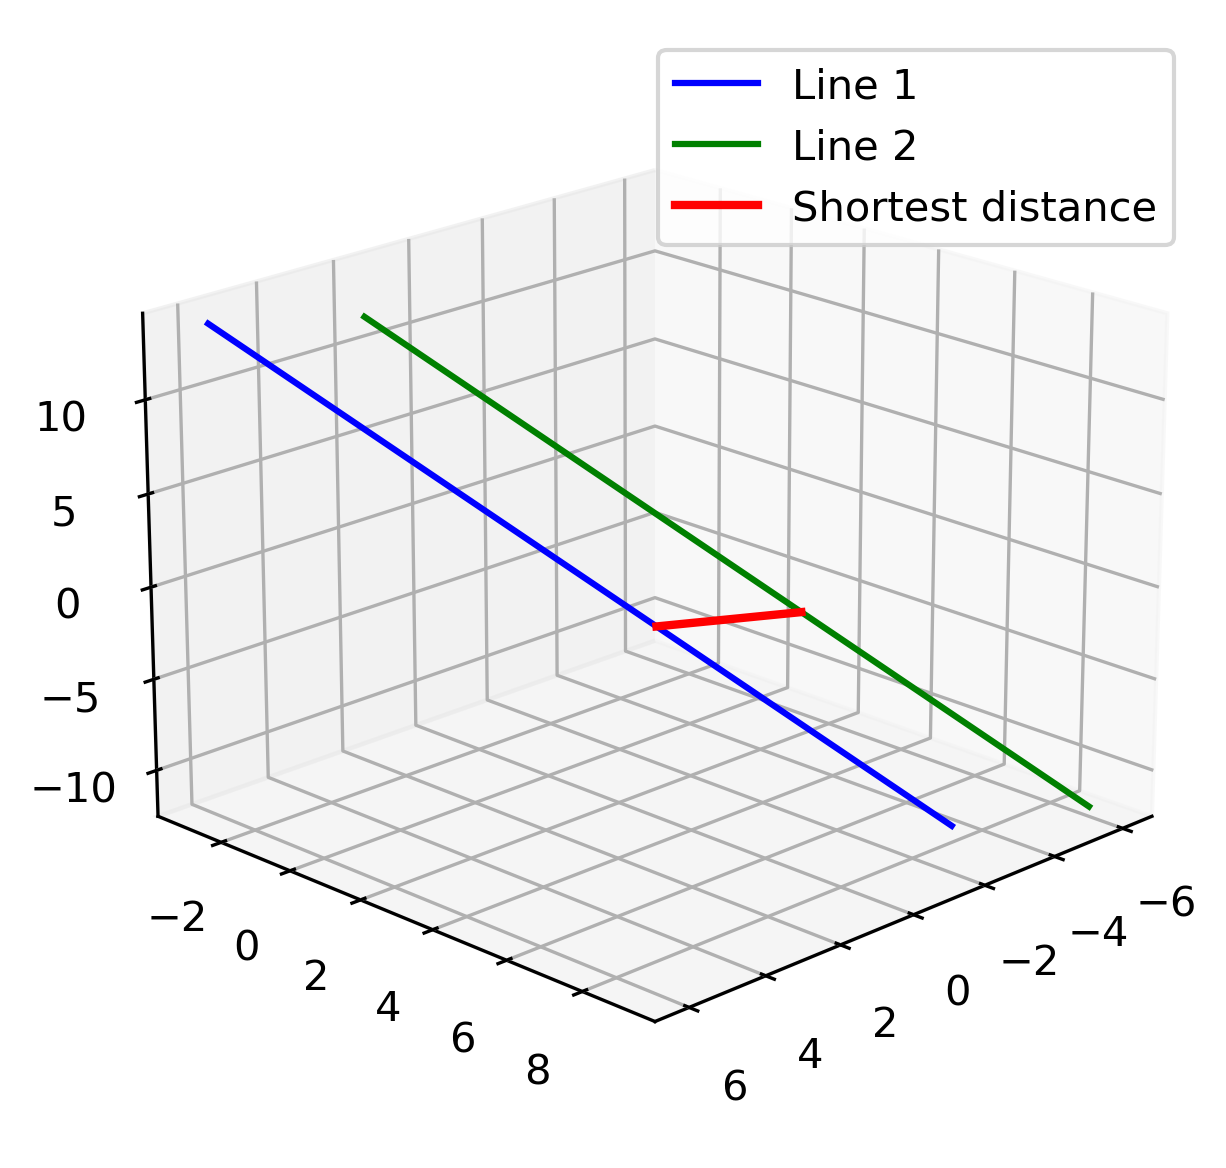
\includegraphics[width=0.7\linewidth]{figures/shortest_distance.png}
    \caption{Shortest distance between two parallel lines}
    \label{fig:placeholder}
\end{figure}

jhuj

\end{frame}

\end{document}
